\section{事業化・社会実装の具体的な進め方}

\subsection{本提案で開発する製品・サービスのビジネスモデルまたは社会実装のサービスモデル}

本プロジェクトの社会実装のサービスモデルは,OSSとしてソースコードを公開し,かつ
リリースバージョンのバイナリを配布することで世界中の誰でもが自由にサービスを利用・評価し,
自ら改善や提案ができるようにする.また,\ref{section:objective}で述べたとおり,
ユーザと3Dアプリケーション開発者からなるエコシステムを形成することがこのプロジェクトの
1つの目的であり,それによって個人レベルの開発者が作業環境としてのXRを改善し,
ユーザがその恩恵を受けつつ,そこに新しい市場を生む世界を目指している.

また,事業継続のための収益化のため,助成金やクラウドファンディングによる金銭的支援と,
その対価として,作業空間としてのXR空間を改善していくことや,ビジネス展開として
法人向けにZIGENを用いたXR作業環境をハードウェアの準備から,その後のサポートまで一貫して提供する
サービスの提供を考えている.

\subsection{事業期間中の事業化・社会実装に向けての作業内容}
\label{section:biz-plan-detail}

\subsubsection*{ユーザと3Dアプリケーション開発者からなるエコシステムを形成する.}

世界中の開発者やユーザを巻き込めるようにDiscordやGitHubの言語を英語に統一し,
開発の手順をまとめたドキュメントをホスティングする.

\subsubsection*{多くのユーザに使ってもらう.}

まずは認知度を高めるためにカンファレンスやイベント,メディアに積極的に露出し,情報を発信する.
具体的なイベントなどの候補の例は以下のようなものである.
XR Kaigi\footnote{XR Kaigi 2021:https://xrkaigi.com/2021},
XR Kaigi mini\footnote{XR Kaigi mini:https://yellow-haircut-be9.notion.site/XR-Kaigi-mini-209b9db4ad734d17ad65f2321aaf5b09},
CES\footnote{CES:https://www.ces.tech/},
XR Creative Award 2021\footnote{XR Creative Award:https://xrc.or.jp/award2021/},
Digital Content Expo\footnote{Digital Content Expo:https://www.dcexpo.jp/exhibition/}.
またすでに現時点での開発成果をSIGGRAPH2022のEmerging Technologiesに申請済みである.
これらの活動はエコシステムの形成や,コミュニティでのプレゼンスを高めるという目標にも寄与する.

また提供するドキュメントが適切で,ユーザが自立的にZIGENを試せる状況であるかについては
ユーザテストを行い,ドキュメントやセットアップ方法などにフィードバックしていきたい.

\subsubsection*{XR世界を作り上げているコミュニティでのプレゼンスを高める.}

GitHubが提供しているOSSプロジェクトのガイドラインなどを参考にOSSコミュニティとしての完成度を
高める.具体的にはテストやドキュメント,Code of Conduct,マイルストーンなどの整備である.
またこれはOSS向けのFoundationに助成金を申請する場合にも重要である.

\subsubsection*{事業の継続のための収益化について.}

助成金やクラウドファンディングについての具体的な作業内容は,まずどのFoundationなどを
ターゲットにするか決め,それに対して対価の設計をし,申請することである.

ビジネス展開については,普段から仕事でLinuxデスクトップを利用している開発者,そうでない開発者,
非開発者などの属性それぞれについてZIGENでの作業環境に移行する可能性があるか
ユーザインタビューを行い検証していきたい.

\subsection{作業体制}

木内:主にOSSとしての完成度向上に取り組む.
江口:主に事業継続のための収益化に取り組む.
伴:主にカンファレンスやイベントなどの準備に取り組む.
劉:テストやドキュメントに関して取り組む.
渡辺:主に全体のバックアップとして取り組む.

なお渡辺に関しては未踏ジュニア\footnote{未踏ジュニア:https://jr.mitou.org/}に
応募しており未踏ジュニアに採択時には本プロジェクトへの参加を取りやめる予定であり,
その場合はバックアップメンバがいなくなる.

\subsection{作業線表}

図\ref{fig:biz-schedule}に示した.

\begin{figure}[htbp]
  \centering
  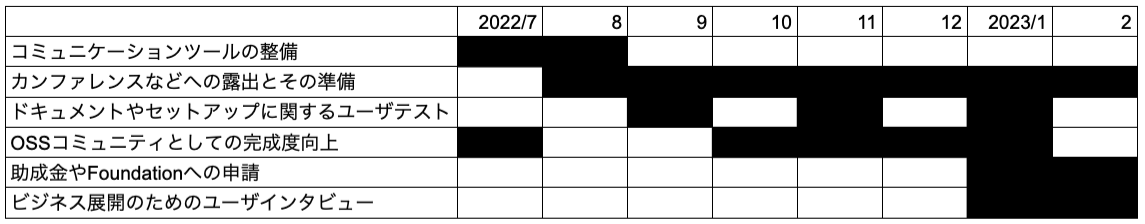
\includegraphics[keepaspectratio, width=\linewidth]{fig/biz-schedule.png}
  \caption{作業線表.黒塗りの時期が取り組む時期.}
  \label{fig:biz-schedule}
\end{figure}

\subsection{克服すべき課題とその解決策}

克服すべき課題はビジネス展開において,Linux デスクトップユーザやHMD保持者の絶対数が少ないこと
である.そのための施策として,HMDやLinux デスクトップPCなどのハードウェアを含めた
XR作業環境一式を提供するサービスを考えている.このときに普段からLinuxユーザを使っている開発者,
そうでない開発者,非開発者がそれぞれどれほど,XRでのLinuxデスクトップ環境を受け入れ,
使ってゆく可能性があるのかはユーザインタビューを通して検証していきたい.

% ・事業化・社会実装の進め方について、以下の項目を記述してください。
% - 本提案で開発する製品・サービスのビジネスモデルまたは社会実装のサービスモデル
% - 事業期間中の事業化・社会実装に向けての作業内容(事業化体制の構築、マーケティン
% グ等)
% - 作業体制:目標を達成できる体制になっているか。チームの場合はコミットされた役割
% 分担等も記載してください。他の未踏事業に応募しているメンバーがいる場合、その
% メンバーが抜けた場合の体制についても記載してください。
% - 作業線表(スケジュール)
% - 克服すべき課題とその解決策
